\scanpage{86}
% archive foliation: 85
X\quad 1\qquad exists (and is unique) in quasi coherent case.
State that $\mathcal E$ is of finite type (resp. finite
presentation \inserted{or loc. free}) iff $\mathcal E_1,\mathcal E_2$ are.

\margin{\unsure{d}}
5
\margin{$+S_3$}
\figure{
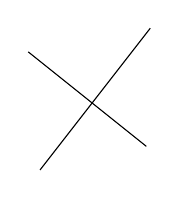
\begin{tikzpicture}
\draw (0,1.5)--(1.5,0.3);
\draw (0.15,0)--(1.55,1.8);
\end{tikzpicture}
}

12\quad Amounts to showing: \deleted{\unsure{$X$}}
\unsure{finite|fnt} flat covering of $S$
is tame with r. to $D_1,D_2$ iff it \deleted{\unsure{is so}}
restriction to $S_1,S_2$ are tamely ramified.
\uline{Should be trivial} with the conditions considered!
